%!TEX root = ../../secondYearReport.tex

\subparagraph{Extension and enhancement of the iDyn library. (T1.5)}

Goal of this task is to provide a reliable software tool for on-line estimation of whole-body dynamics. Before CoDyCo, dynamic estimations on the iCub were relying on the iDyn software library\footnote{\url{https://github.com/robotology/icub-main/tree/master/src/libraries/iDyn}.}, designed for  fixed-base robots. Within the first year of CoDyCo, iDynTree\footnote{{\url{https://github.com/robotology/codyco/tree/master/src/libraries/iDynTree}}.} was released in response to the need of representing floating base structures. During the second year of the project, we investigated on the problem of extending iDynTree to the case of multiple redundant sensors. The investigation resulted in an experimental software library\footnote{\url{https://github.com/iron76/bnt_time_varying}.} currently implemented in \textsc{Matlab}. The software performs maximum-a-posteriori dynamic estimation fusing multiple sensors such as gyroscopes, linear accelerometers, embedded force-torque sensors and encoders. Computational efficiency is obtained by exploiting the sparsity of the underlying problem \cite{Nori2015} (see Fig.~\ref{fig:varTimeComplete}). Estimation accuracy is obtained by a modified version of the expectation maximisation algorithm \cite{Nori2015b} (see Fig.~\ref{fig:extForceEstimation}). 

\begin{figure}
  \centering 
	  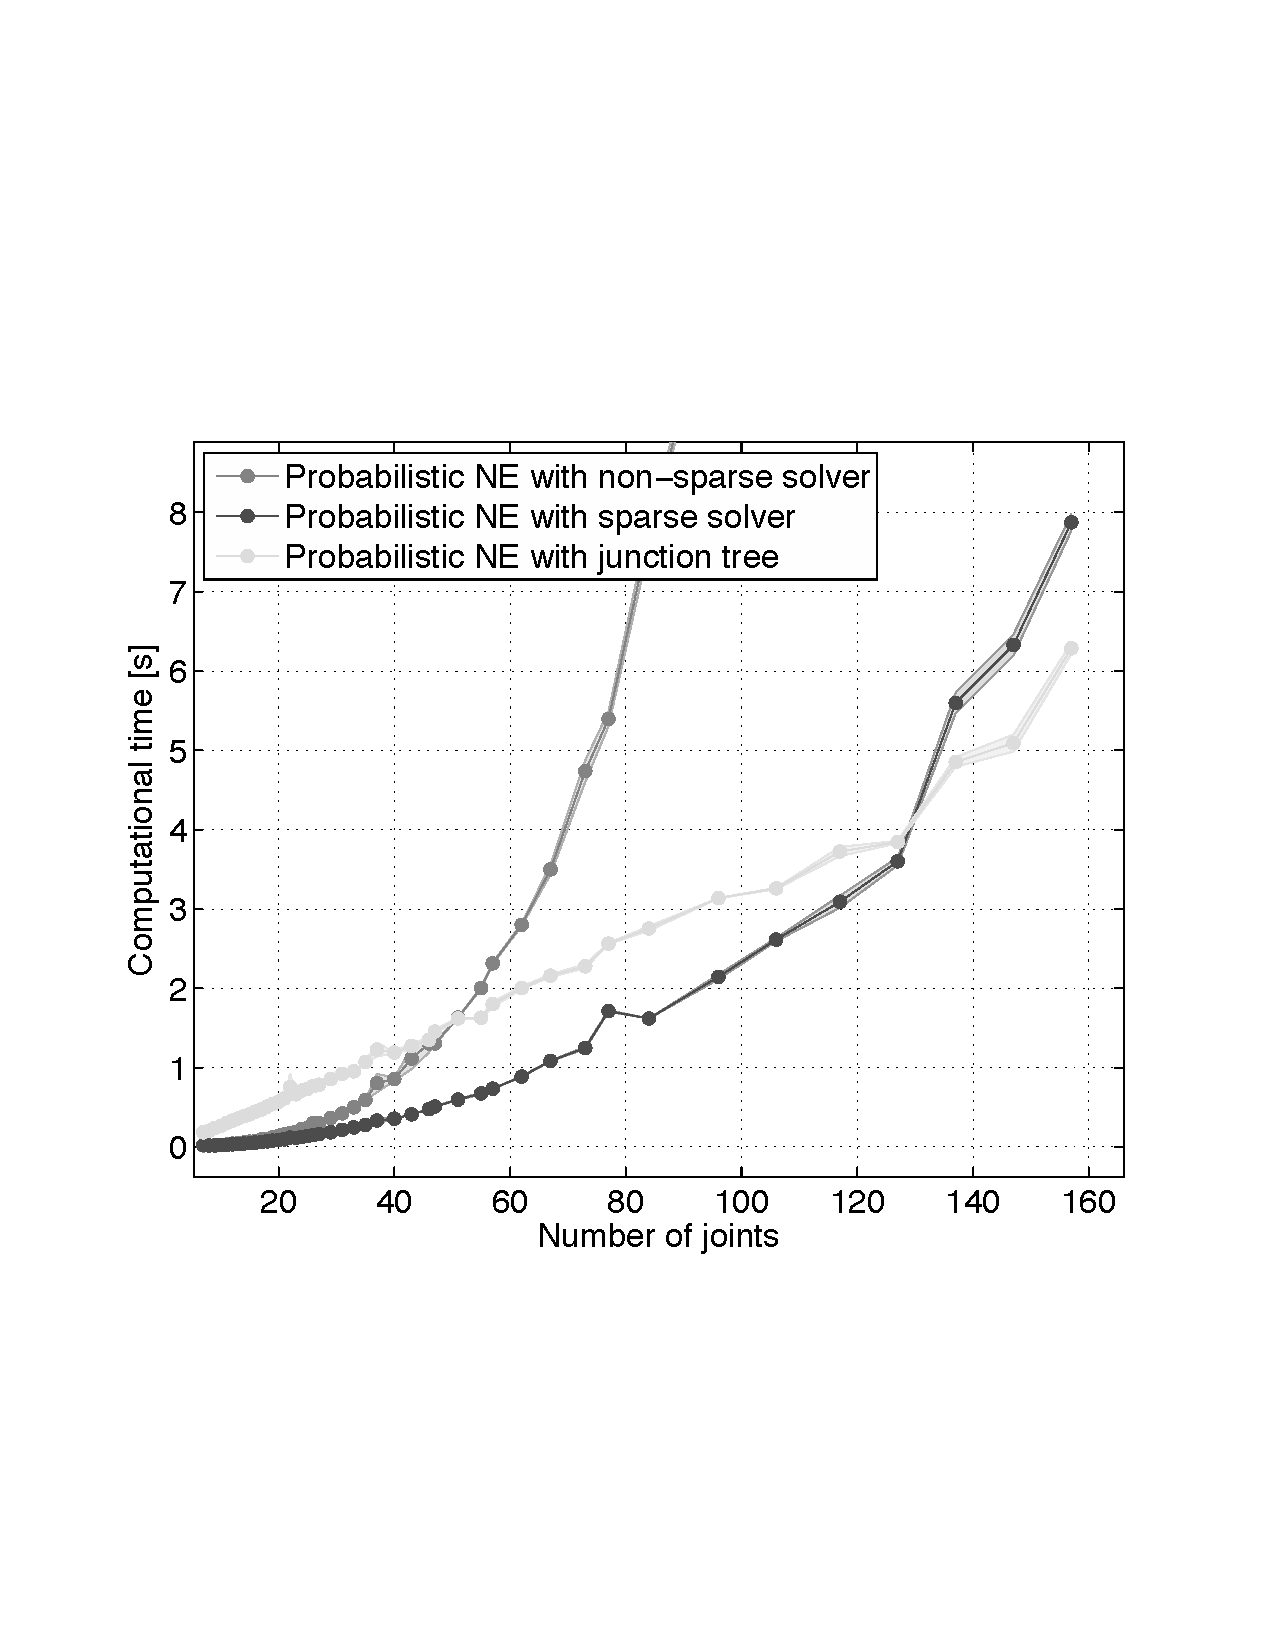
\includegraphics[height=0.35\hsize]{images/varTimeComplete.pdf} 
\caption{\label{fig:varTimeComplete} Comparison of non-sparse (S1-gray), sparse (S2-dark-gray) and Bayesian network junction tree (S3-light-gray) solvers in solving maximum-a-posteriori dynamics with redundant measurements (see \cite{Nori2015} for details).}
\end{figure}

\begin{figure*} [!ht]
  \centering 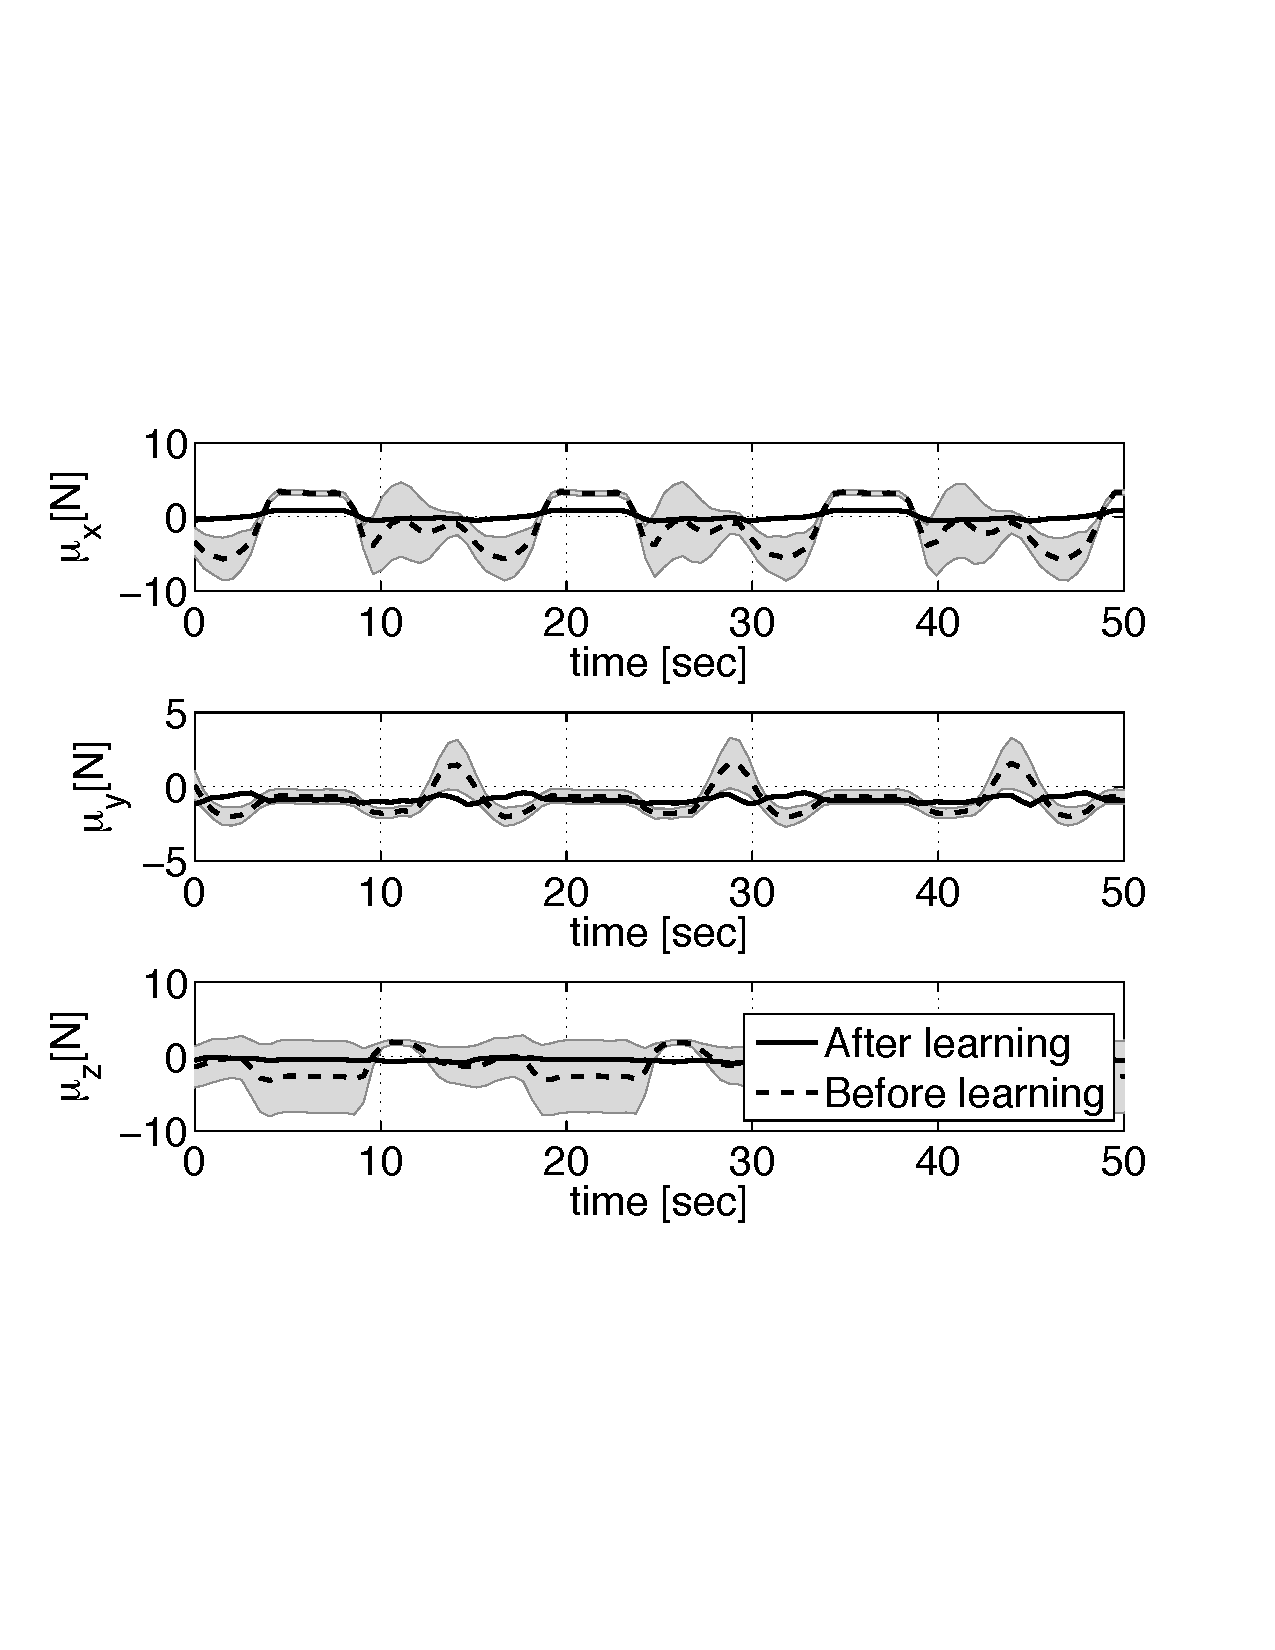
\includegraphics[width=0.45\hsize]{images/torques.pdf}  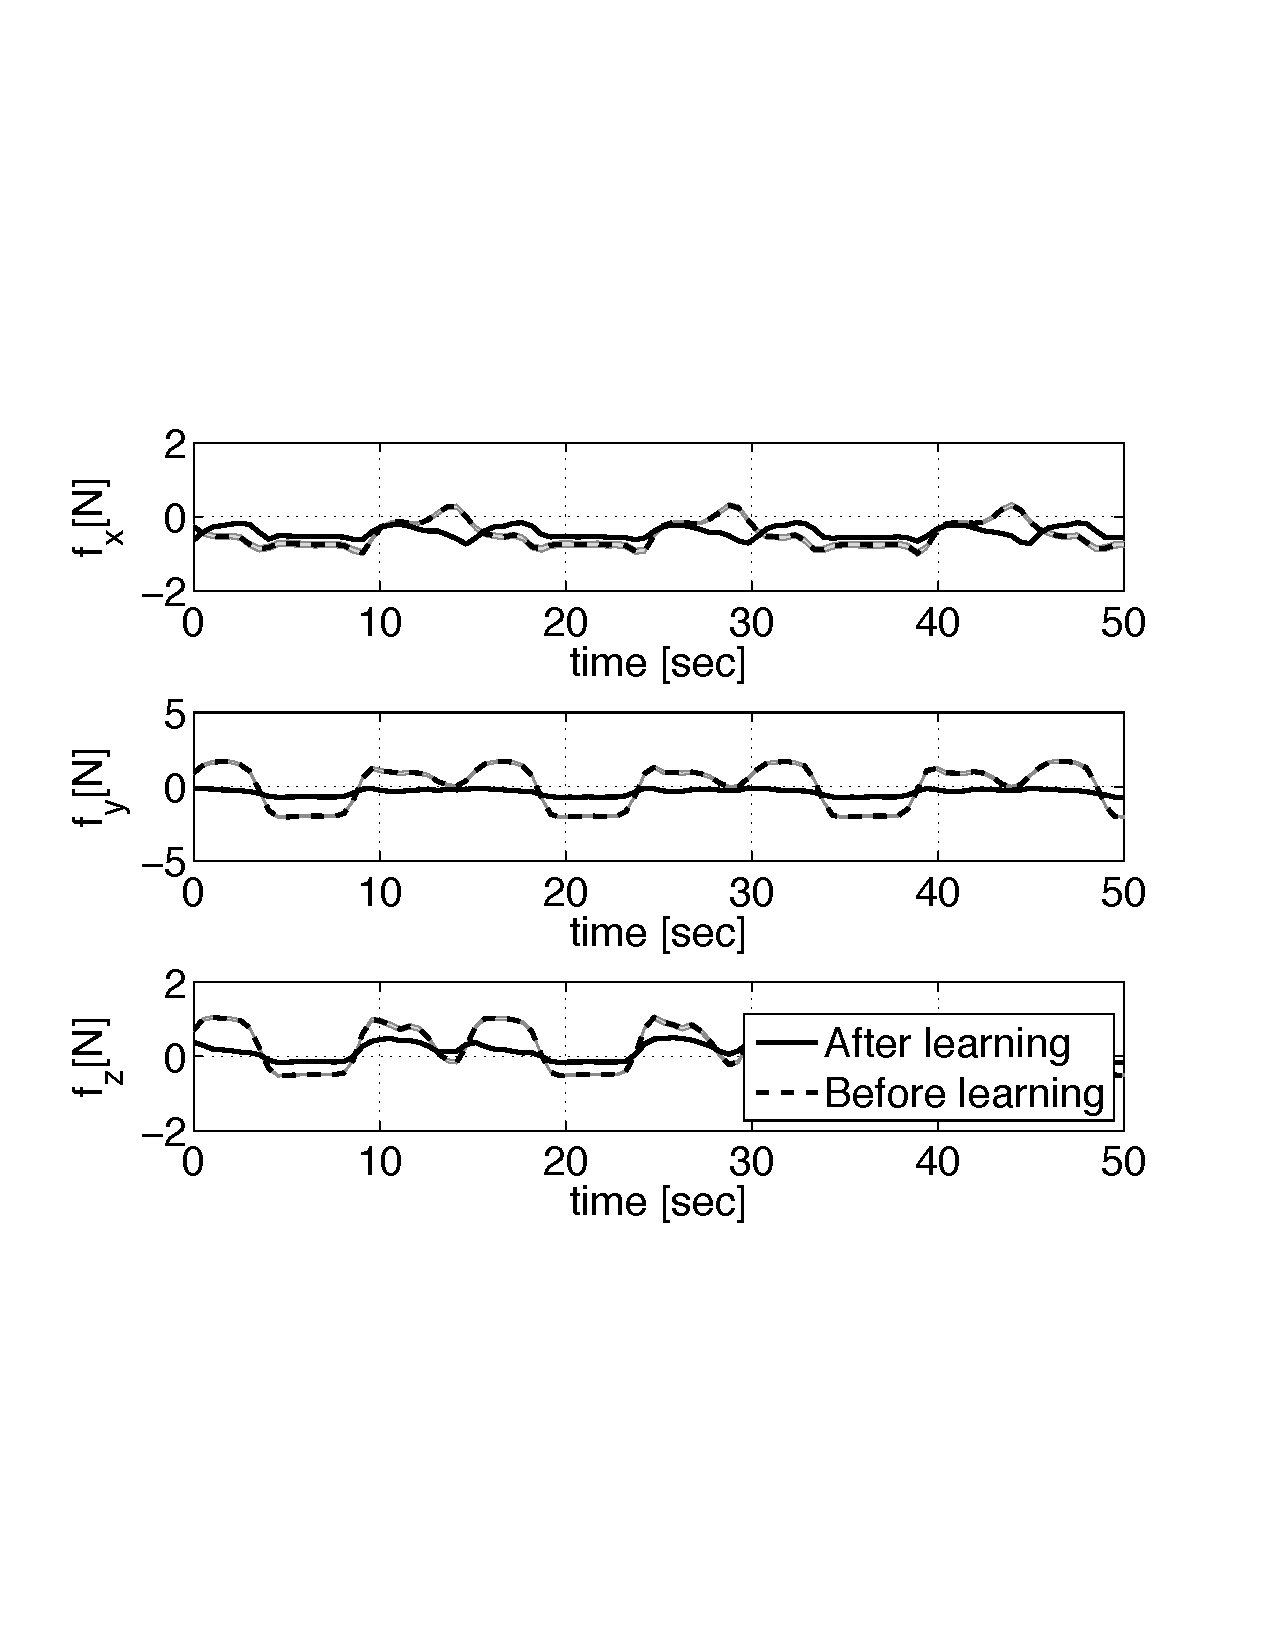
\includegraphics[width=0.45\hsize]{images/forces.pdf} 
\caption{\label{fig:extForceEstimation} The picture shows the errors in estimating an external wrench. The two curves refer to the estimation obtained before (dashed line) and after (solid line) the estimation of the data covariance with a modified EM algorithm \cite{Nori2015b}.}
\end{figure*}




